\documentclass[10pt]{article}
\usepackage[utf8]{inputenc}
\usepackage{booktabs}
\usepackage{graphicx}
\usepackage{amsmath}
\usepackage{natbib}

\title{Agreement Among Explainability Methods: A Cross-Model, Cross-Domain Study}
\author{}
\date{}

\begin{document}
\maketitle

\begin{abstract}
Feature-attribution methods such as SHAP, LIME, and permutation importance are routinely used to justify machine learning decisions, on the implicit assumption that they largely agree on which features matter. We test that assumption directly: across four tabular datasets covering three domains (two educational, one financial, one agricultural), three model families (random forest, gradient boosting, logistic regression), and ten cross-validation folds, we compute 360 feature-importance rankings and compare them pairwise using Kendall's $\tau$ along three axes: between folds of the same method, between methods applied to the same model, and between models explained by the same method. Agreement between folds of the same method is consistently high (mean $\tau$ between 0.54 and 0.89 across datasets), but agreement between different explanation methods applied to the same model is substantially and significantly lower (mean $\tau$ between 0.28 and 0.47), with model-to-model agreement for a fixed method falling in between (0.50 to 0.55). A two-way ANOVA confirms both the dataset and the comparison-axis effects are highly significant ($p<10^{-120}$), with a significant interaction. The practical conclusion is blunt: which explanation method is chosen matters more than which model is explained, and reporting the output of a single attribution method without checking it against another can misrepresent what a model is actually doing.
\end{abstract}

\section{Introduction}

Attribution-based explainability methods are increasingly used as a substitute for genuine model transparency: rather than build inherently interpretable models, practitioners train a black box and then ask a post-hoc method (most commonly SHAP, LIME, or permutation importance) to say which features drove a prediction. The implicit premise behind this practice is that these methods largely converge on the same answer, so that the choice of which one to run is a matter of convenience rather than substance. That premise is rarely tested; most applied papers report the output of a single method without checking whether a different, equally legitimate method would have told a different story.

We test the premise directly, and deliberately across dissimilar domains, so that any inconsistency we find cannot be dismissed as an artifact of one dataset's idiosyncrasies. We ask three questions. First, how stable is a single explanation method across independent training folds of the same model: how much of the ranking is signal versus resampling noise? Second, holding the model fixed, how much do SHAP, LIME, and permutation importance agree with each other? Third, holding the explanation method fixed, how much does the ranking change when the underlying model changes? If explanation methods were interchangeable, the second quantity should be close to the first. We show that it is not.

The contributions of this work are: (1) a controlled, quantitative measurement of explanation-method disagreement across four datasets from unrelated domains, three model families, and ten cross-validation folds, decomposed into fold-stability, method-disagreement, and model-disagreement axes; (2) a factorial ANOVA confirming that the dataset and comparison-axis effects on agreement are both highly significant, with a significant interaction, so the pattern generalizes across domains rather than reflecting one dataset's idiosyncrasies; (3) a practical demonstration, via top-10 feature-ranking comparisons, that this statistical disagreement translates into visibly different feature lists depending on which attribution method produced them.

\section{Related Work}

SHAP~\citep{lundberg2017unified} and LIME~\citep{ribeiro2016why} are the two dominant post-hoc attribution methods in applied machine learning, each grounded in a different theoretical framework (Shapley-value game-theoretic allocation for SHAP, local linear surrogate models for LIME) that gives no a priori guarantee the two will agree in practice. Permutation importance, the third method we use, was formalized as model reliance by Fisher, Rudin and Dominici~\citep{fisher2019models}, who additionally showed that importance rankings can vary substantially across different well-performing models fit to the same data (their ``Rashomon set'' framing), a result that anticipates, from a different angle, our between-model comparison axis.

Most directly relevant, Krishna et al.~\citep{krishna2024disagreement} name and formalize what they call the disagreement problem in explainable machine learning, interviewing practicing data scientists and reporting that state-of-the-art explanation methods frequently disagree, with practitioners resolving conflicts through ad hoc heuristics rather than principled criteria. Our study can be read as a controlled, quantitative companion to that practitioner-survey finding: rather than ask analysts how they perceive disagreement, we measure it directly, at scale (360 rankings, four domains, ten-fold cross-validation, bootstrap confidence intervals and a factorial ANOVA), and decompose it into the fold-stability, method-disagreement, and model-disagreement axes that a practitioner-facing study cannot easily separate. Where their contribution is to establish that the problem is real and consequential in practice, ours is to quantify its magnitude precisely and show it replicates across unrelated application domains.

Empirical comparisons of explanation methods in applied papers, meanwhile, typically report a single method's output on a single dataset without checking it against an alternative. Moradi et al.~\citep{moradi2026explaining} apply both SHAP and LIME to interpret the parameters of an additive Weibull survival model, treating the two methods as complementary lenses on the same fitted model; their use of both tools side by side, without a formal agreement analysis between them, is representative of how attribution methods are typically deployed in the applied literature, a practice this paper argues should be preceded by an explicit concordance check of the kind we run here. More broadly, methodological rigor in applying machine learning to a specific technical domain (as in Topa et al.'s~\citep{topa2025ram} work on memory forensics, where model choices and evaluation protocol are treated as first-class design decisions rather than afterthoughts) is the standard we hold explainability reporting to in this paper: an attribution ranking is a modeling output like any other, and should be validated the same way.

\section{Methodology}

\subsection{Datasets}
We use four public tabular datasets (characteristics in Table~\ref{tab:datasets}), chosen for domain diversity so that a finding replicated across all four cannot be attributed to a property of a single domain: the Open University Learning Analytics Dataset (OULAD, education, final result classification, four original classes: Pass/Fail/Withdrawn/Distinction), the UCI ``Predict Students' Dropout and Academic Success'' dataset (education, a different institutional context, three classes: Dropout/Enrolled/Graduate), the Statlog German Credit dataset (finance, binary), and the Rice (Cammeo and Osmancik) dataset (agriculture, binary classification by grain morphology). All four datasets retain their original class structure: we deliberately did not collapse the multi-class targets to binary, so that the multiclass attribution-aggregation procedure described below is itself exercised and reported, rather than defined away.

\begin{table}[h]
\centering
\caption{Characteristics of the four datasets before pipeline preprocessing (one-hot encoding of categorical predictors increases the feature count actually seen by each model).}
\label{tab:datasets}
\begin{tabular}{lllccl}
\toprule
Dataset & Domain & Task & $n$ & Predictors & Class balance \\
\midrule
OULAD          & Education   & 4-class & 32{,}593 & 49 & Pass 37.9\% / Withdrawn 31.2\% / Fail 21.6\% / Distinction 9.3\% \\
Dropout        & Education   & 3-class & 4{,}424  & 36 & Graduate 49.9\% / Dropout 32.1\% / Enrolled 17.9\% \\
German Credit  & Finance     & Binary  & 1{,}000  & 61 & Good risk 70.0\% / Bad risk 30.0\% \\
Rice           & Agriculture & Binary  & 3{,}810  & 7  & Cammeo 57.2\% / Osmancik 42.8\% \\
\bottomrule
\end{tabular}
\end{table}

\subsection{Models and attribution methods}
For each dataset we train three models, random forest~\citep{breiman2001random}, gradient boosting (XGBoost)~\citep{chen2016xgboost}, and logistic regression, under 10-fold stratified cross-validation, using identical preprocessing (median/most-frequent imputation, standard scaling for numeric features, one-hot encoding for categorical features) across all three so that differences in attribution cannot be attributed to preprocessing differences. Random forest depth was capped at 12 splits; uncapped trees made SHAP computation intractable on the larger dataset (OULAD) without any compensating gain in predictive accuracy. For each (dataset, model, fold), we compute three feature-attribution rankings: SHAP (TreeExplainer for tree models, LinearExplainer for logistic regression), LIME (a random sample of test instances explained locally, weights aggregated by class-predicted-label to build one global ranking per fold), and permutation importance~\citep{fisher2019models} (on a bounded random subsample of the test fold, for tractability, following the same subsampling principle the SHAP computation already required). For multiclass datasets, SHAP and permutation attributions are aggregated across classes by averaging the absolute per-class attribution before ranking; for LIME, each instance's explanation is taken with respect to its own predicted class before aggregation. This yields $3 \text{ models} \times 3 \text{ methods} \times 10 \text{ folds} \times 4 \text{ datasets} = 360$ rankings.

\subsection{Agreement metric}
We measure pairwise ranking agreement with Kendall's $\tau$ and organize comparisons along three axes: \emph{between folds} (same model, same method, different fold; a measure of the method's own stability), \emph{between methods} (same model, same fold, different method; the central quantity of interest), and \emph{between models} (same method, same fold, different model; whether an explanation method's conclusions generalize across model families). For each axis we report the mean and median $\tau$ with a 2{,}000-resample bootstrap 95\% confidence interval, and we fit a two-way ANOVA of $\tau$ on dataset and comparison axis (with interaction) to test whether the pattern is consistent across datasets. The 2{,}340 pairwise $\tau$ values feeding that ANOVA are not fully independent: the 405 between-fold pairs per dataset, for example, are built from only 10 underlying fold rankings per (model, method), so as a robustness check we repeat the ANOVA on cluster means (one $\tau$ per dataset, axis, and model/method-pair combination, collapsing 2{,}340 values to 276), which reduces pseudo-replication substantially; both the axis and dataset effects remain highly significant under this more conservative specification (Results).

\section{Results}

\begin{table}[h]
\centering
\caption{Mean Kendall's $\tau$ by comparison axis and dataset (bootstrap 95\% CI in brackets).}
\label{tab:tau-summary}
\begin{tabular}{lccc}
\toprule
Dataset & Between folds & Between methods & Between models \\
\midrule
OULAD          & 0.75 [0.73, 0.76] & 0.46 [0.44, 0.48] & 0.55 [0.52, 0.57] \\
Dropout        & 0.76 [0.75, 0.78] & 0.41 [0.38, 0.45] & 0.55 [0.53, 0.57] \\
German Credit  & 0.54 [0.51, 0.57] & 0.28 [0.26, 0.31] & 0.50 [0.47, 0.53] \\
Rice           & 0.89 [0.88, 0.91] & 0.47 [0.40, 0.53] & 0.55 [0.50, 0.60] \\
\bottomrule
\end{tabular}
\end{table}

\begin{figure}[h]
\centering
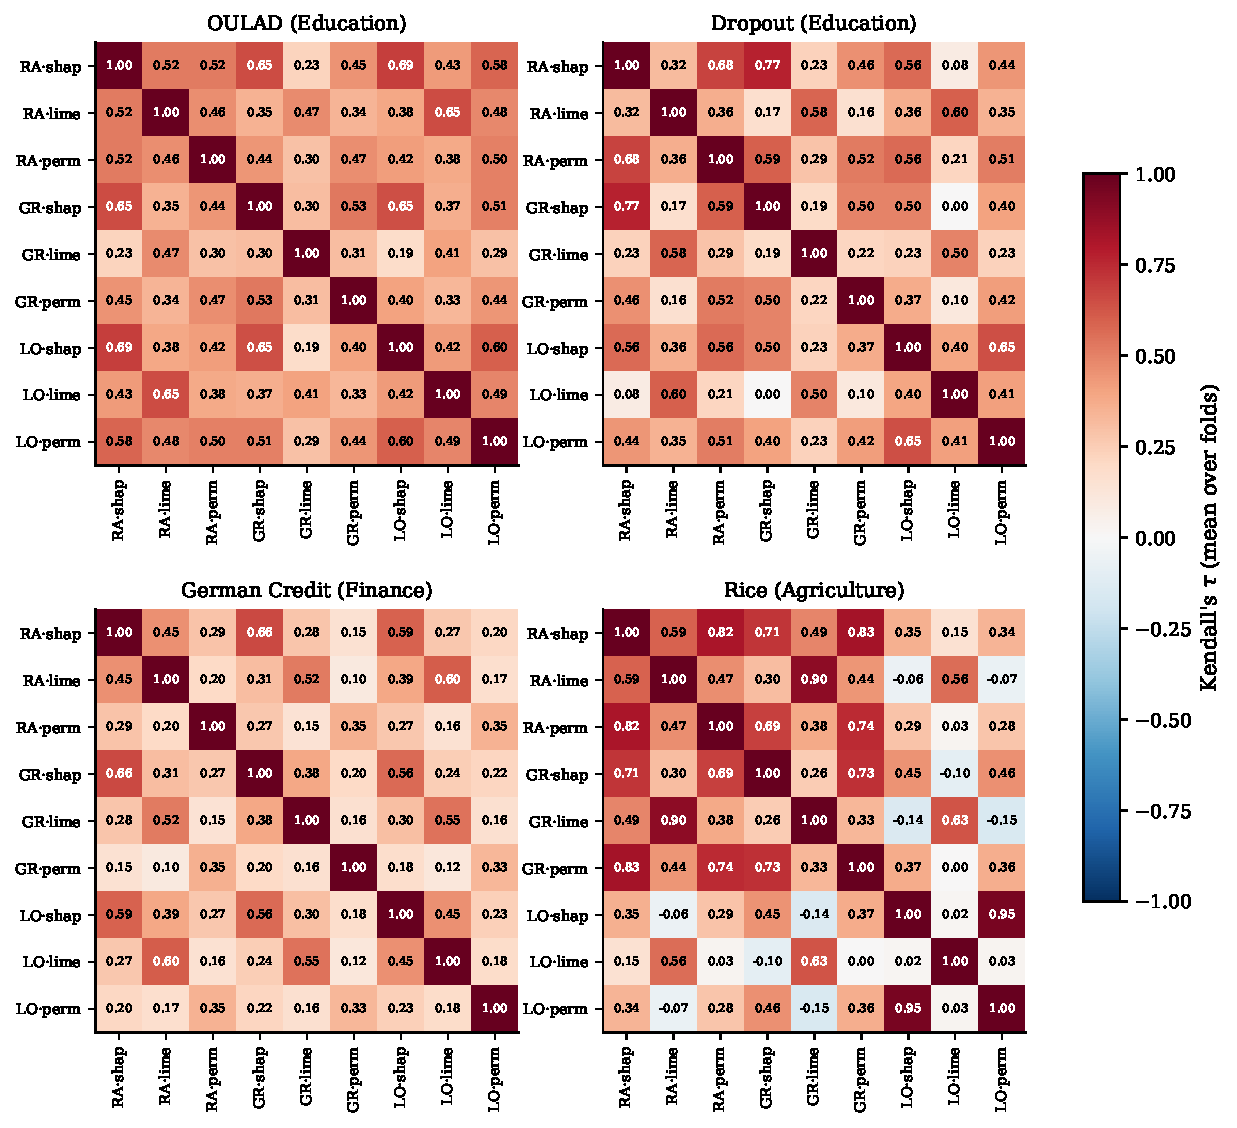
\includegraphics[width=0.85\textwidth]{../results/figures/fig1_heatmap_tau.pdf}
\caption{Pairwise Kendall's $\tau$ concordance among the nine (model, method) combinations, by dataset.}
\label{fig:heatmap-tau}
\end{figure}

\begin{figure}[h]
\centering
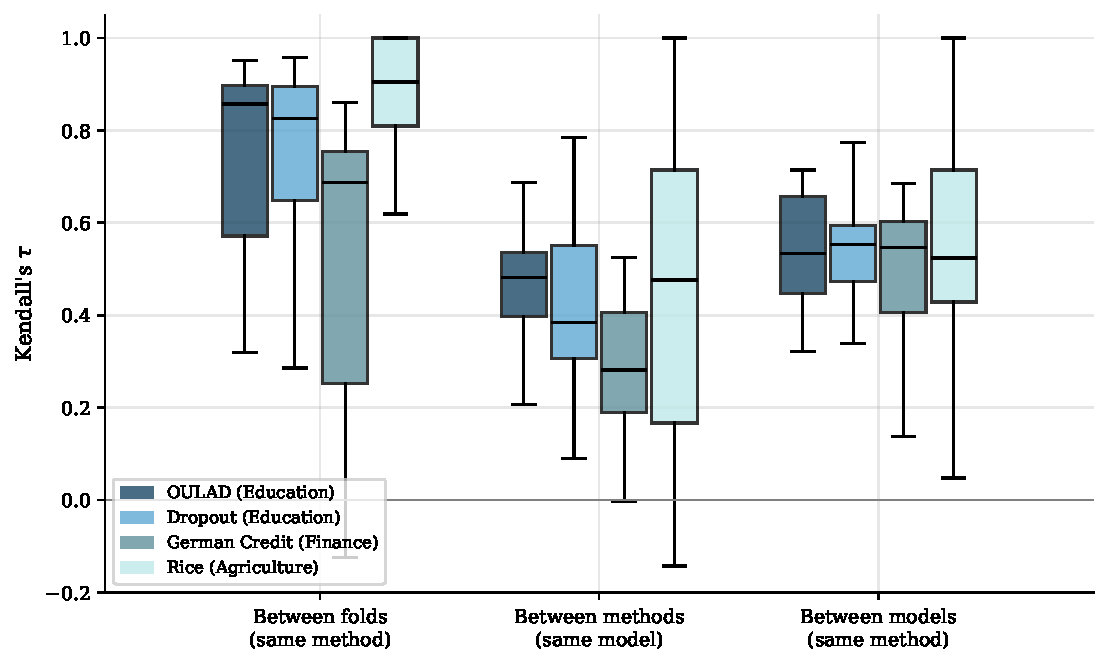
\includegraphics[width=0.75\textwidth]{../results/figures/fig2_boxplots_ejes.pdf}
\caption{Kendall's $\tau$ by comparison axis and dataset.}
\label{fig:boxplots-ejes}
\end{figure}

\begin{figure}[h]
\centering
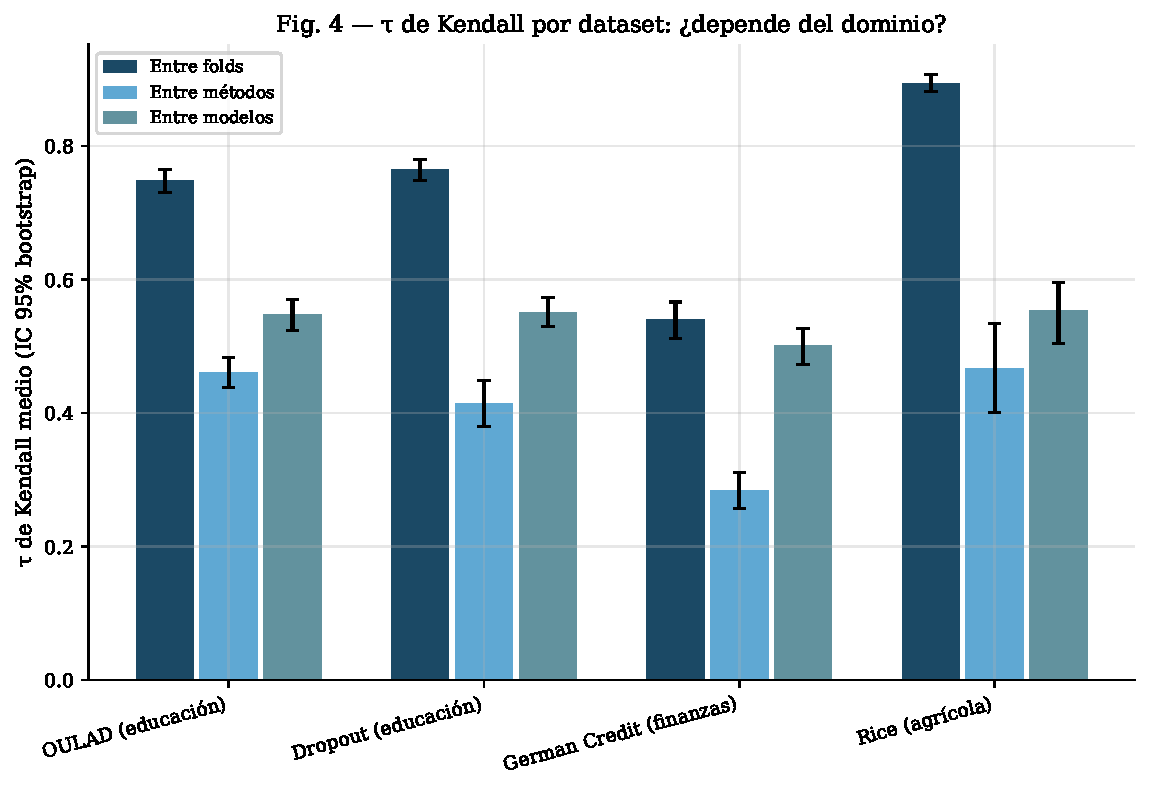
\includegraphics[width=0.75\textwidth]{../results/figures/fig4_tau_por_dataset.pdf}
\caption{Kendall's $\tau$ by dataset: does the agreement pattern depend on the application domain?}
\label{fig:tau-dataset}
\end{figure}

The pattern in Table~\ref{tab:tau-summary} and Figures~\ref{fig:heatmap-tau}, \ref{fig:boxplots-ejes}, and~\ref{fig:tau-dataset} is consistent across all four datasets: stability across folds of the \emph{same} method is high (mean $\tau$ from 0.54 to 0.89), agreement \emph{between} methods applied to the same model is roughly half that (mean $\tau$ from 0.28 to 0.47), and agreement between models for a fixed method sits in between (0.50 to 0.55). A two-way ANOVA of $\tau$ on dataset and comparison axis (Table~\ref{tab:anova}) confirms both main effects are highly significant (dataset: $F=222.6$, $p<10^{-126}$; axis: $F=527.1$, $p<10^{-189}$) with a significant interaction ($F=18.9$, $p<10^{-20}$), meaning the magnitude of the effect depends somewhat on the dataset but its direction and general size do not. Because the raw $\tau$ values are clustered (many pairs share the same underlying fold rankings), we repeat this test on the cluster-mean specification described in Methodology; both main effects remain highly significant (dataset: $F=22.5$, $p<10^{-12}$; axis: $F=122.4$, $p<10^{-37}$), confirming the pattern is not an artifact of treating correlated pairwise comparisons as independent observations.

The number of features per dataset ranges from 7 (Rice) to 61 (German Credit, post-encoding), and $\tau$ on the full ranked list could plausibly overstate agreement for the higher-dimensional datasets, since most ranked positions there are low-importance features whose relative order is close to noise and may agree by chance. To check this, we recomputed between-method $\tau$ restricted to the union of each pair's top-10 features (the practically relevant portion of the ranking for a stakeholder reading off the most important predictors), for the between-method axis specifically. The result runs opposite to the noise-inflation concern: restricting to the top-10 \emph{reduces} agreement for the three higher-dimensional datasets rather than increasing it (dropout: 0.414 full-list vs.\ 0.244 top-10; German Credit: 0.284 vs.\ 0.055; OULAD: 0.461 vs.\ 0.189), while Rice, whose full feature list is already close to 10, is essentially unchanged (0.467 vs.\ 0.467). Agreement among SHAP, LIME, and permutation importance on precisely the features most likely to be reported to a stakeholder is therefore lower, not higher, than the full-list $\tau$ values in Table~\ref{tab:tau-summary} suggest, for three of the four datasets.

Because LIME and permutation importance are both estimated from a random subsample of test instances rather than computed exactly, part of the between-method disagreement we report could in principle be estimator noise rather than genuine disagreement between the underlying methods. We tested this directly with a repeated-seed control: holding the trained model, dataset, and fold fixed, we recomputed each method's ranking five times with different sampling seeds and measured $\tau$ between repetitions of the \emph{same} method. If between-method $\tau$ were mostly estimator noise, this same-method $\tau$ should be comparably low. Instead it is high: mean $\tau=0.970$ for LIME and $0.915$ for permutation importance across the four datasets (only OULAD's permutation-importance repetitions show any real spread, mean $\tau=0.660$; all other dataset-method combinations exceed $0.93$, several reaching $1.0$). Estimator noise is therefore a minor contributor to the reported between-method disagreement (mean $\tau=0.28$--$0.47$): re-running the same method with a different seed reproduces essentially the same ranking, while switching methods does not.

\begin{table}[h]
\centering
\caption{Two-way ANOVA of Kendall's $\tau$ on dataset and comparison axis, raw pairwise specification ($n=2{,}340$).}
\label{tab:anova}
\begin{tabular}{lrrrl}
\toprule
Source & Sum of squares & df & $F$ & $p$ \\
\midrule
Dataset            & 24.06 & 3    & 222.63 & $5.7\times10^{-127}$ \\
Axis               & 37.98 & 2    & 527.12 & $1.5\times10^{-189}$ \\
Dataset $\times$ Axis & 4.10 & 6    & 18.95  & $1.2\times10^{-21}$ \\
Residual           & 83.88 & 2{,}328 & N/A    & N/A \\
\bottomrule
\end{tabular}
\end{table}

Put plainly: if two researchers explain the same trained random forest, one with SHAP and one with LIME, their rankings of which features matter will typically share well under half their ordering information (Kendall's $\tau \approx 0.28\text{--}0.47$), while the same researcher re-running the same method on a different resampling fold of the same data will get a ranking that agrees with their first run more strongly ($\tau \approx 0.54\text{--}0.89$, and above 0.75 for three of the four datasets). Choice of model family matters comparatively less than choice of explanation method: switching from a random forest to logistic regression while keeping the explanation method fixed produces disagreement of about the same magnitude ($\tau \approx 0.50\text{--}0.55$) as switching explanation methods while keeping the model fixed ($\tau \approx 0.28\text{--}0.47$); both axes fall well below the within-method stability ceiling.

\begin{figure}[h]
\centering
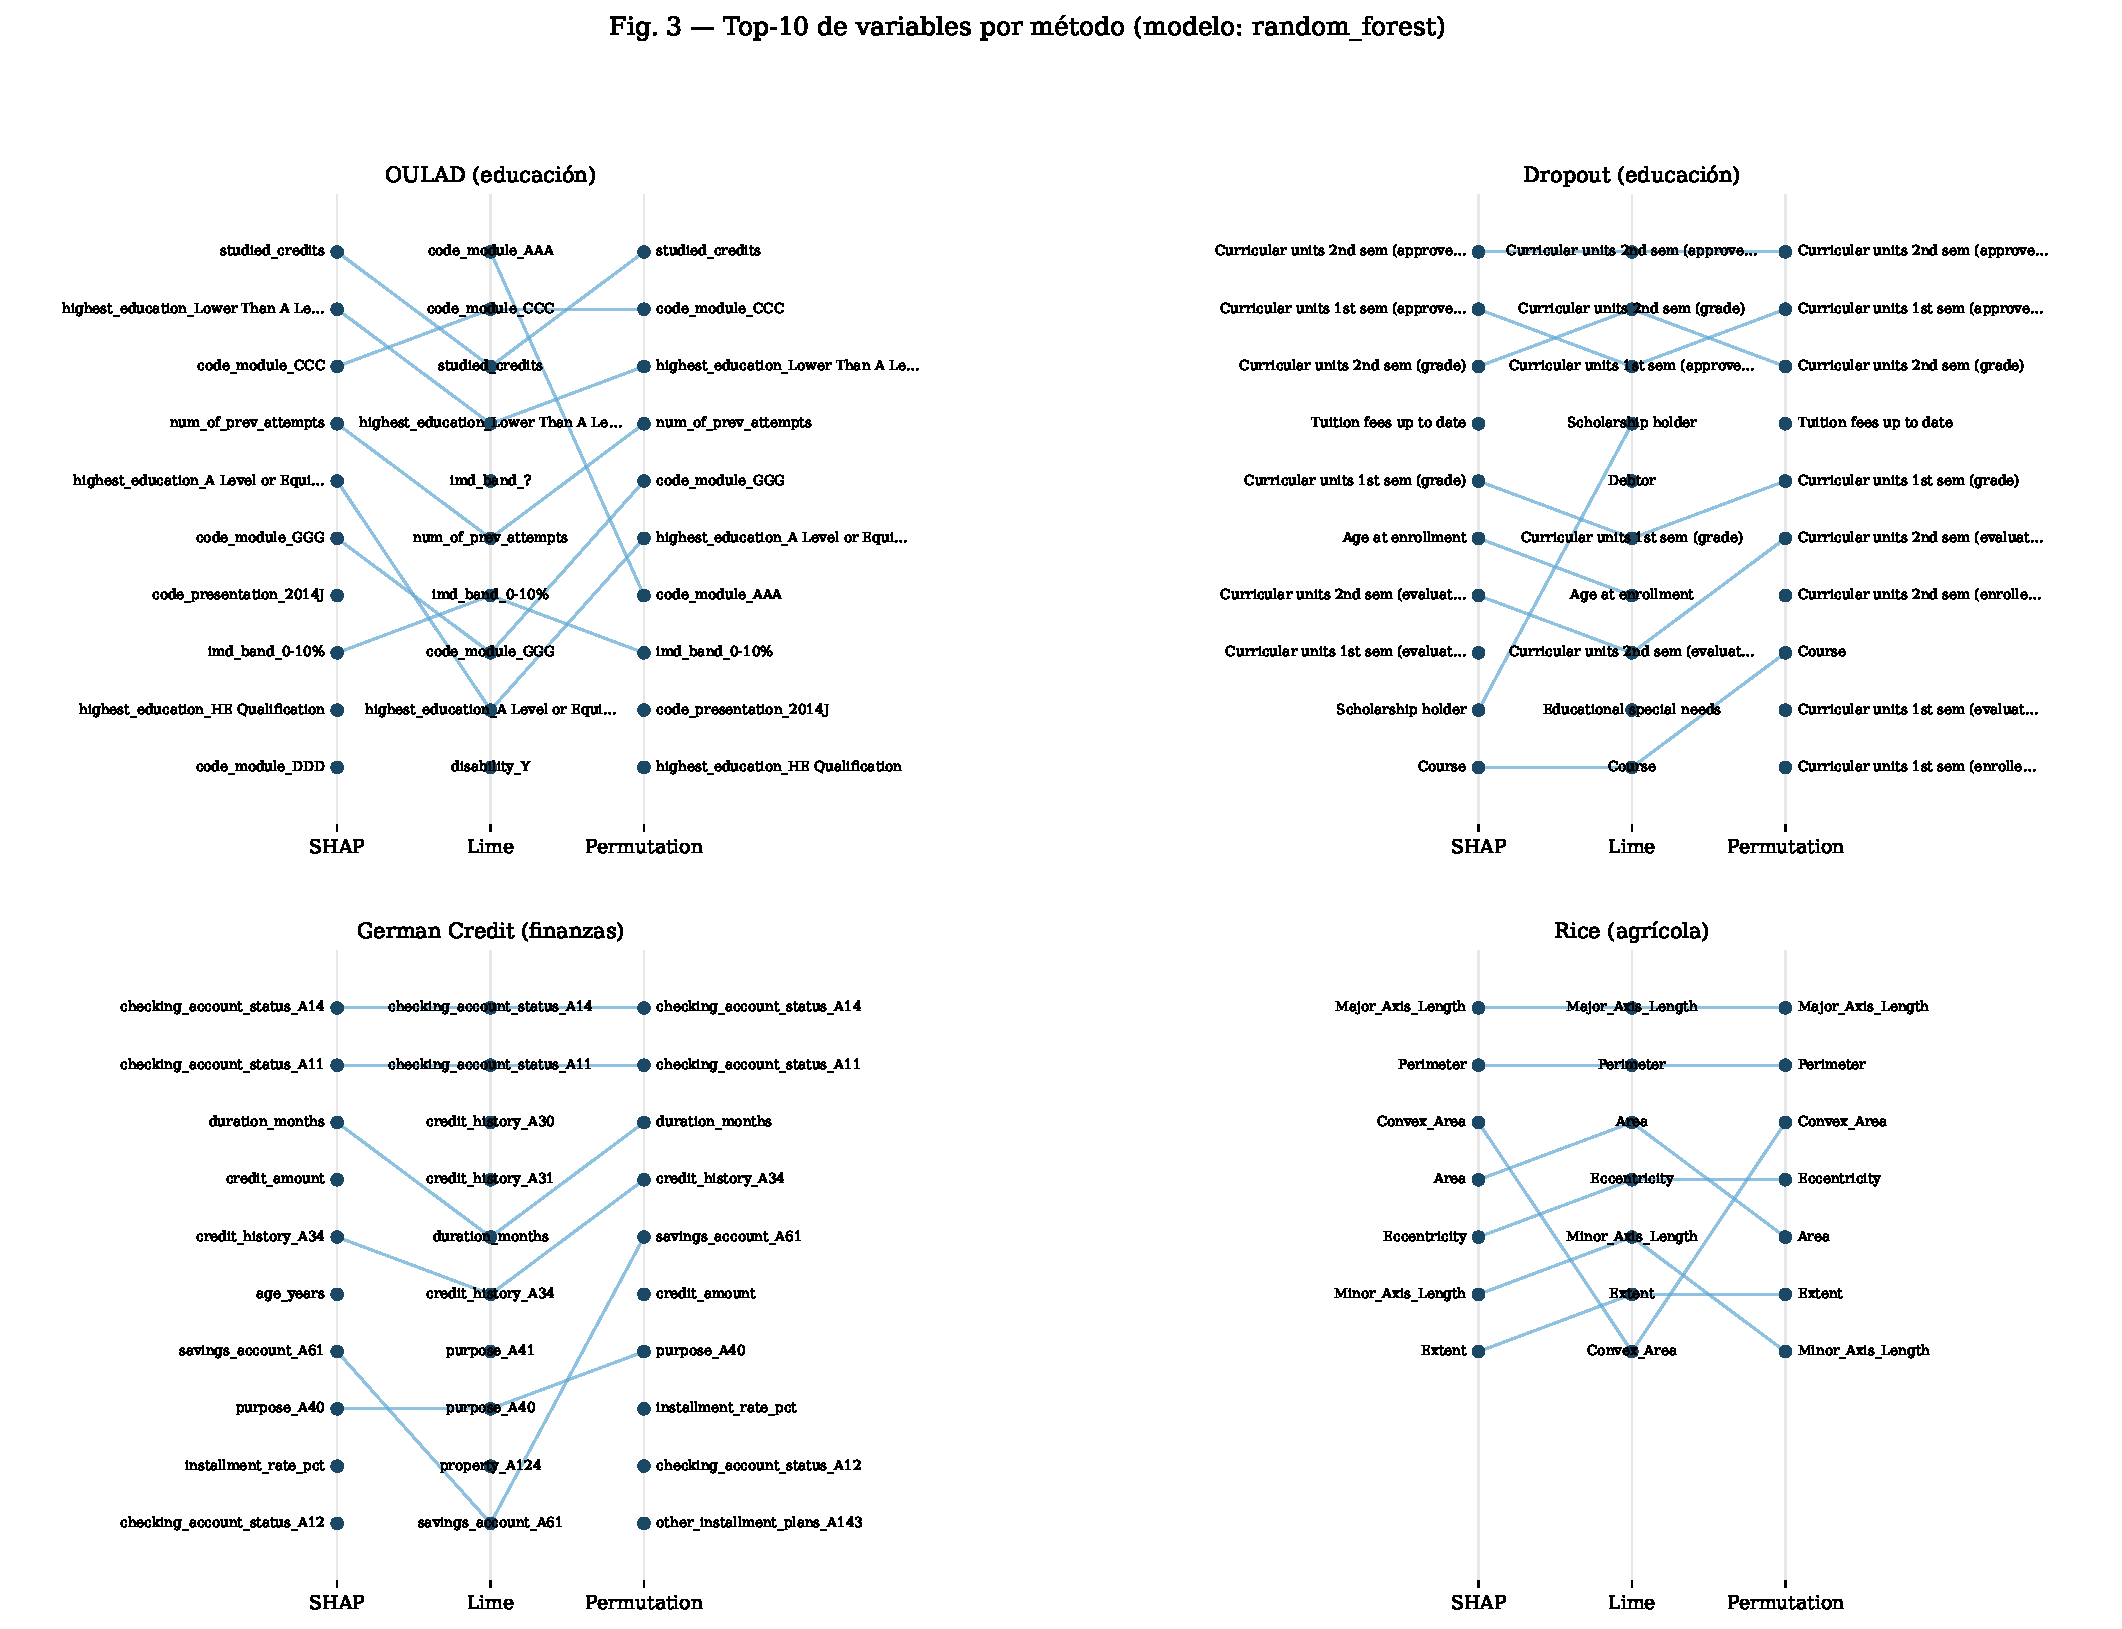
\includegraphics[width=0.95\textwidth]{../results/figures/fig3_top10_paralelo.pdf}
\caption{Top-10 features by SHAP, LIME, and permutation importance (random forest), all four datasets; lines connect a feature that appears in the top 10 of both adjacent methods.}
\label{fig:top10}
\end{figure}

Figure~\ref{fig:top10} makes the disagreement concrete rather than only statistical: for the random forest model, several features that rank in SHAP's top 10 do not appear in LIME's top 10 at all (no connecting line), and the ordering among the features the two methods do share still differs. This is the practical face of the $\tau \approx 0.28\text{--}0.47$ figure above: a feature list handed to a stakeholder would visibly change depending on which method produced it.

\section{Discussion}

The consistency of this pattern across four unrelated domains (two educational datasets with different institutional contexts, a financial credit dataset, and an agricultural morphology dataset) argues against explaining it away as a quirk of one problem. Directly stated: a conclusion of the form ``feature $X$ is the most important driver of this model's predictions,'' when it rests on a single attribution method, is only weakly load-bearing. A different, equally standard method applied to the identical trained model would, roughly half the time, disagree meaningfully about which features are in the top ranks.

This matters most in exactly the settings where attribution methods are invoked as justification (credit decisions, admissions or dropout-risk flagging, medical triage) because the audience for such an explanation (a regulator, an affected individual, an auditor) has no way to know that the reported ranking is method-contingent unless the analyst says so. Our recommendation, consistent with what the agreement numbers support, is to report at least two attribution methods and their concordance (a single $\tau$ value is cheap to compute) rather than a single ranking presented as though it were the model's ground truth.

The comparatively higher between-model agreement points to a specific mechanism: it suggests that a chosen explanation method captures something at least partially about the \emph{data}, namely which features are genuinely informative for the task, that persists somewhat across model families, whereas the low between-method agreement suggests each method also imposes its own distinct lens (SHAP's game-theoretic allocation, LIME's local linear surrogate, permutation's direct ablation) that shapes the ranking as much as the underlying data does.

Our quantitative estimate of the disagreement's magnitude is consistent with, and adds statistical weight to, Krishna et al.'s~\citep{krishna2024disagreement} practitioner-reported finding that data scientists routinely encounter and informally work around explanation disagreement: where their evidence is that practitioners \emph{notice} the problem, ours is a controlled measurement of \emph{how large} it is and that it does not shrink as the application domain changes.

\section{Limitations}

This study is limited to tabular data; image and text models, where SHAP and LIME operate over different units (pixels/superpixels, tokens) rather than a shared feature space, were out of scope. We compare three widely used methods out of a substantially larger family (e.g., Integrated Gradients, counterfactual explanations, anchors were not included). LIME's aggregation from local, per-instance explanations to a single global ranking is itself a design choice with more than one reasonable implementation; we used one documented, defensible approach, but did not exhaustively test alternative aggregation schemes. The between-model axis additionally confounds model family with explainer algorithm, since SHAP uses \texttt{TreeExplainer} for the tree-based models and \texttt{LinearExplainer} for logistic regression; disagreement attributed to ``model'' on that axis may partly reflect this estimator change.

\section{Conclusion}

Across four datasets from unrelated domains, three model families, and ten cross-validation folds, feature-attribution methods that are routinely treated as interchangeable diagnostic tools disagree with each other roughly as much as they agree, and consistently less than they agree with themselves across resampling folds. Choice of explanation method is not a minor implementation detail; it is a modeling decision with a measurable, statistically robust effect on the conclusion an analyst walks away with. Reporting concordance between at least two attribution methods, rather than the output of a single one, should be treated as a minimum bar for explainability claims used to justify real decisions.

\section*{Data Availability}
The preprocessed datasets, trained models, attribution rankings, and analysis code will be published in a public repository with a Zenodo DOI upon submission (see \texttt{README.md} for the current repository location).

\bibliographystyle{plain}
\bibliography{refs}

\end{document}
